\section{Output}
Depending on application, different output formats might come in handy. PET
supports three output options:

\begin{description}
    \item[plain]\hfill\\
        The example in \autoref{lst:pet_output_plain} shows the simple
        \emph{plain}-format, which is a simple output format intended for
        use as input for further processing.
    \item[table]\hfill\\
        The table format, with an example shown in \autoref{lst:pet_output_table},
        shows a terminal-printable output which is easier to understand by
        humans, and is intended for further study of the numbers. This might
        come in handy as the last format, GNUPlot-graph, might be hard to
        read when you are out after very specific information.
    \item[graph]\hfill\\
        This last format is the default, and will try to give an overview of
        the entire program in a easy digestible format. An example of such
        a graph is printed in \autoref{fig:annot}.
\end{description}

The output format is understood as timeslots in which the architecture
has a certain current drain, which should be multiplied with applied voltage to
get numbers on consumed energy, heat generation and so on. The numbers are
scaled as milliamperes, which of course is equal to milliwatt if voltage is
$1V$. PET displays its output as mA as it was easier to find current drain
rather than wattage using our test bench. Current can be found measuring the
voltage drop of the core supply rail over a shunt resistor, finding wattage meant that we also had
to monitor the exact voltage drop over the entire circuit, correlate these numbers in time, and
multiply them together.

It is known from Ohms law in \autoref{eq:ohm} and the definition of electric power in \autoref{eq:power}

\begin{equation}
I=\frac{U}{R}
\label{eq:ohm}
\end{equation}

\begin{equation}
P=U \cdot I
\label{eq:power}
\end{equation}

that power equals current squared times resistance:

\[U=R \cdot I\]
\[P=(R \cdot I) \cdot I\]
\[P=I^2 \cdot R\]
and that power equals voltage squared divided by resistance:
\[P=U \cdot \frac{U}{R}\]
\[P=\frac{U^2}{R}\]

Thus, measuring the current drain as amperes means that energy consumption will be
very dependent on values like resistance and voltage, but these are not yet known,
and the result will have to be scaled proportionally as voltage and resistance becomes
known.


All output formats supports annotation of function calls. This is achieved by
giving PET a list of symbols and their corresponding program counter value. PET
will tag each power bucket with the last seen symbol within that bucket, as this
symbol is the one most likly to continue over to the next measure point. Lists
of symbols can be extracted from non-stripped binaries using the script listed
in \autoref{lst:annotscript}. This script is also included in the \texttt{scripts}-folder
of PET.

\lstinputlisting[float,label={lst:annotscript},caption={Extract symbols from binary},language=sh]{../pet/scripts/annotate.sh}

Example of the \texttt{plain} output format can be seen in
\autoref{lst:pet_output_plain}. The left column is the bucket number, while the
right column is instant current draw from the modelled architecture.

\begin{lstlisting}[float,label={lst:pet_output_plain},caption={PET Plain Output}]
0 120 memcpy
1 113 start
2 150 main
3 123 main
4 133 fun1
5 117 main
\end{lstlisting}

When reading the output directly from console, a more descriptive output format
is the \texttt{table} format. An example using this option is rendered in
\autoref{lst:pet_output_table}.

\begin{lstlisting}[float,label={lst:pet_output_table},caption={PET Table Output}]
/----------------------------------------\
|   Bucket   |  milliAmps |    Symbol    |
|------------|------------|--------------|
|          0 | 120.000000 |    memcpy    |
|          1 | 113.000000 |    start     |
|          2 | 150.000000 |    main      |
|          3 | 123.000000 |    main      |
|          4 | 133.000000 |    fun1      |
|          5 | 117.000000 |    main      |
\----------------------------------------/
\end{lstlisting}

Visualization is often a good thing when inspecting old or trying to understand
new problems. As it is hard to get a good overview from huge text log files, PET
provides, as stated in \autoref{subsec:annot}. In effect, it is formatting
temporary output files and calling GNUPlot do do the hard work.

\begin{figure}
    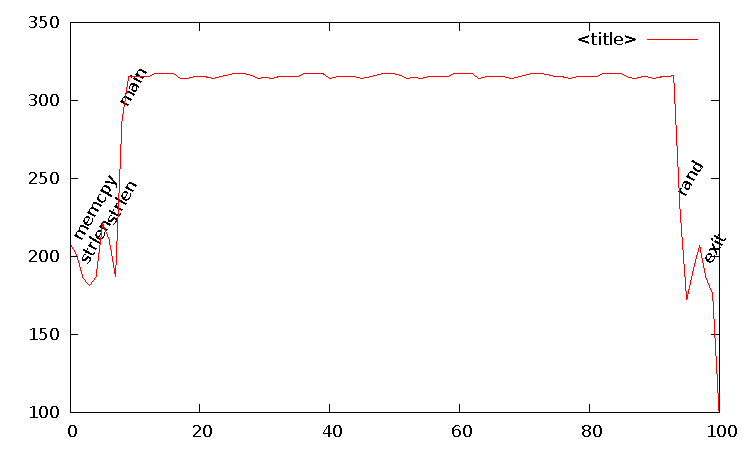
\includegraphics[width=0.9\textwidth]{figs/annot.pdf}
    \caption{PET Annotated Graphical Output}
    \label{fig:annot}
\end{figure}

